\chapter{Theory}

\section{Magnetic ordering}
\subsection{Domains}
To understand the origin of ultrafast dynamics in magnetically ordered systems we first need to understand what domains are.
They are defined as regions of uniform direction of the order parameter, in the case of ferromagnets it is the magnetization.
This splitting of the magnetic structure into different domains is caused by the minimization of the free energy in the material.
There are several energy contributions coming into play.
Only when they balance out eachother, a stable magnetic state of the sample is possible.
The first and foremost term involved in the forming of domains is the field energy $E_{\text{f}}$ stored in form of the magnetostatic field around the sample.
A large domain also generates a large magnetic field as the field energy scales with the square of the domain size.
Therefore to reduce the field energy the material is split into domains of ever smaller size.
But this shrinking of the domain sizes does not go on indefinetely.
One of the opposing energy terms is the domain wall energy $E_{\text{D}}$ and scales with the root of the domain size.
At the boundries between different domains, which are called domain walls, neighbouring magnetic moments are forced to point in opposite directions.
This goes against the exchange interaction trying to align the magnetic moments in the same direction and there is a energy cost associated with it.
So the domain size is mostly determined by the balance of the field energy saved by domain splitting and the energy cost of additional domain walls.

A further reduction of the field energy is brought on by neighbouring domains having orthogonal magnetizations.
The involved domains are then called flux closure domains.
As the name implies trough the orthogonal arrangement of the domains the field loops get closed almost entirely inside the material.
Since magnetic media have an easy direction of magnetization, flux closure domains result in the magnetization of some domains to be at an angle to this easy direction.
This introduces two additional energetic costs to the equation.
Having the orientation of magnetization at an angle to the easy axis causes an energy term, the magnetocrystalline anisotropy energy $E_{\text{mc}}$, to arise as it is more energetically favourable to have the magnetic moments to align parallel to the easy axis.
The magnetoelastic anisotropy energy $E_{\text{me}}$ is another term caused by a deviation of the orientation of magnetization from the easy axis.
% As a consequence the magnetic dipoles, meaning the ions, deform slightly which induces tiny mechanical stresses on the sample and thus the emerging of such a domain comes with an energy cost.
As a consequence the magnetic dipoles, meaning the ions, deform slightly which induces tiny mechanical stresses on the sample, leading to a phenomenon labeled magnetostriction.
This culminates in an energy cost hindering the emergence of such closure domains at an angle to the easy axis.

All of these odds in the form of energy costs are stacked against non-parallel alignment which means that most of the volume in a magnetic material holds domains with their magnetization oriented parallel to the easy direction.
This equation
\begin{equation}
    E_{\text{f}} = E_{\text{D}} + E_{\text{mc}} + E_{\text{me}}
    \label{eqn:landau_lifschitz_energy}
\end{equation}


\subsection{Antiferromagnetic domains}

\section{Sample system NiO/C60}
\subsection{NiO}
As Ni is a transition metal it carries some unique properties simplifying possible theoretical calculations and making it especially interesting for fundamental research.
Having only a partially filled 3d-orbital in its electronic structure each Ni-ion possesses a net magnetic moment, caused by the angular momenta associated with the unpaired electrons.
Simplified, both the orbital angular momentum and the spin of an electron create a magnetic moment.
The difference to other classes of magnetically ordered elements such as rare earths and actinides is the spatial position of those partially filled shells.
As our object of interest are not single atoms, but crystals containing them, the interaction of the electrostatic crystal field with the orbital motion of the electron is not to be dissmissed.
Rare earths and actinides having their partially filled orbitals (4f and 5f) screened by outer lying shells experience the crystal field interaction as relatively weak.
Whereas the transition metalls outermost orbitals are exactly those unfilled shells.
This leads to their orbital angular momentum being quenched, so that only the magnetic moments of the spin attributes to the net magnetic moment of the ions.
These spins couple through the so-called exchange interaction which has a purely quantum mechanical in nature and has no classical analogon.
This term in the potential energy originates from the indistinguishability of electrons and the electrostatic interaction between them.
Now this phase transition from the magnetically unordered or more precisely the paramagnetic phase happens by going beneath a transition temperature, where the long range coupling mechanism between the single magnetic moments prevails against the thermally driven disorder.

Thus a distinction can be made between three types of ordered states.
Firstly, the ferromagnetic order, where all magnetic dipole moments are aligned parallel which entails a macroscopic net magnetization.
The more complex structure of ferrimagnetically ordered crystals contains two sublattices pointing in opposite directions.
If the magnetic moments in the two sublattices are of different absolute values there is also a net magnetization present albeit weaker then in ferromagnets.
A special but all the more intriguing case of ferrimagnetism is the antiferromagnetic order.
Here the antiparallel magnetic dipoles from the two sublattices show the same strength.
Consequently, there is no net magnetization present as the oppositely alinged magnetic moments cancel out eachother on a microscopic scale.
Hence there is a need for a new order parameter.
Since the magnetization is easily comprehensible as the density of magnetic dipoles $\vec{m}$ represented by an axial vector
\begin{equation}
    \vec{M} = \frac{\text{d}\vec{m}}{\text{d} V} \;,
\end{equation}
the order parameter for antiferromagnets is derived from it.
This parameter is called staggered magnetization and is defined as the normalized difference between the respective magnetizations of the two sublattices
\begin{equation}
    \vec{M}_{\text{st}} = \frac{\vec{M_1} - \vec{M_2}}{|\vec{M_1} - \vec{M_2}|} \;.
\end{equation}
\begin{figure}[ht]
    \centering
    \includegraphics[width=\textwidth]{pictures/magnetic_order.png}
    \caption{Schematic depiction of transmission pump-probe measurement.}
    \label{fig:pump_probe}
\end{figure}

\subsection{C60}

\section{Magnon dynamics}

\section{Exciton-Magnon-Transition}

